% Options for packages loaded elsewhere
\PassOptionsToPackage{unicode}{hyperref}
\PassOptionsToPackage{hyphens}{url}
\PassOptionsToPackage{dvipsnames,svgnames,x11names}{xcolor}
%
\documentclass[
  letterpaper,
  DIV=11]{scrartcl}

\usepackage{amsmath,amssymb}
\usepackage{iftex}
\ifPDFTeX
  \usepackage[T1]{fontenc}
  \usepackage[utf8]{inputenc}
  \usepackage{textcomp} % provide euro and other symbols
\else % if luatex or xetex
  \usepackage{unicode-math}
  \defaultfontfeatures{Scale=MatchLowercase}
  \defaultfontfeatures[\rmfamily]{Ligatures=TeX,Scale=1}
\fi
\usepackage{lmodern}
\ifPDFTeX\else  
    % xetex/luatex font selection
\fi
% Use upquote if available, for straight quotes in verbatim environments
\IfFileExists{upquote.sty}{\usepackage{upquote}}{}
\IfFileExists{microtype.sty}{% use microtype if available
  \usepackage[]{microtype}
  \UseMicrotypeSet[protrusion]{basicmath} % disable protrusion for tt fonts
}{}
\makeatletter
\@ifundefined{KOMAClassName}{% if non-KOMA class
  \IfFileExists{parskip.sty}{%
    \usepackage{parskip}
  }{% else
    \setlength{\parindent}{0pt}
    \setlength{\parskip}{6pt plus 2pt minus 1pt}}
}{% if KOMA class
  \KOMAoptions{parskip=half}}
\makeatother
\usepackage{xcolor}
\setlength{\emergencystretch}{3em} % prevent overfull lines
\setcounter{secnumdepth}{2}
% Make \paragraph and \subparagraph free-standing
\ifx\paragraph\undefined\else
  \let\oldparagraph\paragraph
  \renewcommand{\paragraph}[1]{\oldparagraph{#1}\mbox{}}
\fi
\ifx\subparagraph\undefined\else
  \let\oldsubparagraph\subparagraph
  \renewcommand{\subparagraph}[1]{\oldsubparagraph{#1}\mbox{}}
\fi

\usepackage{color}
\usepackage{fancyvrb}
\newcommand{\VerbBar}{|}
\newcommand{\VERB}{\Verb[commandchars=\\\{\}]}
\DefineVerbatimEnvironment{Highlighting}{Verbatim}{commandchars=\\\{\}}
% Add ',fontsize=\small' for more characters per line
\usepackage{framed}
\definecolor{shadecolor}{RGB}{241,243,245}
\newenvironment{Shaded}{\begin{snugshade}}{\end{snugshade}}
\newcommand{\AlertTok}[1]{\textcolor[rgb]{0.68,0.00,0.00}{#1}}
\newcommand{\AnnotationTok}[1]{\textcolor[rgb]{0.37,0.37,0.37}{#1}}
\newcommand{\AttributeTok}[1]{\textcolor[rgb]{0.40,0.45,0.13}{#1}}
\newcommand{\BaseNTok}[1]{\textcolor[rgb]{0.68,0.00,0.00}{#1}}
\newcommand{\BuiltInTok}[1]{\textcolor[rgb]{0.00,0.23,0.31}{#1}}
\newcommand{\CharTok}[1]{\textcolor[rgb]{0.13,0.47,0.30}{#1}}
\newcommand{\CommentTok}[1]{\textcolor[rgb]{0.37,0.37,0.37}{#1}}
\newcommand{\CommentVarTok}[1]{\textcolor[rgb]{0.37,0.37,0.37}{\textit{#1}}}
\newcommand{\ConstantTok}[1]{\textcolor[rgb]{0.56,0.35,0.01}{#1}}
\newcommand{\ControlFlowTok}[1]{\textcolor[rgb]{0.00,0.23,0.31}{#1}}
\newcommand{\DataTypeTok}[1]{\textcolor[rgb]{0.68,0.00,0.00}{#1}}
\newcommand{\DecValTok}[1]{\textcolor[rgb]{0.68,0.00,0.00}{#1}}
\newcommand{\DocumentationTok}[1]{\textcolor[rgb]{0.37,0.37,0.37}{\textit{#1}}}
\newcommand{\ErrorTok}[1]{\textcolor[rgb]{0.68,0.00,0.00}{#1}}
\newcommand{\ExtensionTok}[1]{\textcolor[rgb]{0.00,0.23,0.31}{#1}}
\newcommand{\FloatTok}[1]{\textcolor[rgb]{0.68,0.00,0.00}{#1}}
\newcommand{\FunctionTok}[1]{\textcolor[rgb]{0.28,0.35,0.67}{#1}}
\newcommand{\ImportTok}[1]{\textcolor[rgb]{0.00,0.46,0.62}{#1}}
\newcommand{\InformationTok}[1]{\textcolor[rgb]{0.37,0.37,0.37}{#1}}
\newcommand{\KeywordTok}[1]{\textcolor[rgb]{0.00,0.23,0.31}{#1}}
\newcommand{\NormalTok}[1]{\textcolor[rgb]{0.00,0.23,0.31}{#1}}
\newcommand{\OperatorTok}[1]{\textcolor[rgb]{0.37,0.37,0.37}{#1}}
\newcommand{\OtherTok}[1]{\textcolor[rgb]{0.00,0.23,0.31}{#1}}
\newcommand{\PreprocessorTok}[1]{\textcolor[rgb]{0.68,0.00,0.00}{#1}}
\newcommand{\RegionMarkerTok}[1]{\textcolor[rgb]{0.00,0.23,0.31}{#1}}
\newcommand{\SpecialCharTok}[1]{\textcolor[rgb]{0.37,0.37,0.37}{#1}}
\newcommand{\SpecialStringTok}[1]{\textcolor[rgb]{0.13,0.47,0.30}{#1}}
\newcommand{\StringTok}[1]{\textcolor[rgb]{0.13,0.47,0.30}{#1}}
\newcommand{\VariableTok}[1]{\textcolor[rgb]{0.07,0.07,0.07}{#1}}
\newcommand{\VerbatimStringTok}[1]{\textcolor[rgb]{0.13,0.47,0.30}{#1}}
\newcommand{\WarningTok}[1]{\textcolor[rgb]{0.37,0.37,0.37}{\textit{#1}}}

\providecommand{\tightlist}{%
  \setlength{\itemsep}{0pt}\setlength{\parskip}{0pt}}\usepackage{longtable,booktabs,array}
\usepackage{calc} % for calculating minipage widths
% Correct order of tables after \paragraph or \subparagraph
\usepackage{etoolbox}
\makeatletter
\patchcmd\longtable{\par}{\if@noskipsec\mbox{}\fi\par}{}{}
\makeatother
% Allow footnotes in longtable head/foot
\IfFileExists{footnotehyper.sty}{\usepackage{footnotehyper}}{\usepackage{footnote}}
\makesavenoteenv{longtable}
\usepackage{graphicx}
\makeatletter
\def\maxwidth{\ifdim\Gin@nat@width>\linewidth\linewidth\else\Gin@nat@width\fi}
\def\maxheight{\ifdim\Gin@nat@height>\textheight\textheight\else\Gin@nat@height\fi}
\makeatother
% Scale images if necessary, so that they will not overflow the page
% margins by default, and it is still possible to overwrite the defaults
% using explicit options in \includegraphics[width, height, ...]{}
\setkeys{Gin}{width=\maxwidth,height=\maxheight,keepaspectratio}
% Set default figure placement to htbp
\makeatletter
\def\fps@figure{htbp}
\makeatother

<link rel="shortcut icon" href="skript/00-bilder/favicon_bcd_new.svg" />
<link rel="icon" type="image/x-icon" href="logo.ico">
\KOMAoption{captions}{tablesignature}
\makeatletter
\@ifpackageloaded{tcolorbox}{}{\usepackage[skins,breakable]{tcolorbox}}
\@ifpackageloaded{fontawesome5}{}{\usepackage{fontawesome5}}
\definecolor{quarto-callout-color}{HTML}{909090}
\definecolor{quarto-callout-note-color}{HTML}{0758E5}
\definecolor{quarto-callout-important-color}{HTML}{CC1914}
\definecolor{quarto-callout-warning-color}{HTML}{EB9113}
\definecolor{quarto-callout-tip-color}{HTML}{00A047}
\definecolor{quarto-callout-caution-color}{HTML}{FC5300}
\definecolor{quarto-callout-color-frame}{HTML}{acacac}
\definecolor{quarto-callout-note-color-frame}{HTML}{4582ec}
\definecolor{quarto-callout-important-color-frame}{HTML}{d9534f}
\definecolor{quarto-callout-warning-color-frame}{HTML}{f0ad4e}
\definecolor{quarto-callout-tip-color-frame}{HTML}{02b875}
\definecolor{quarto-callout-caution-color-frame}{HTML}{fd7e14}
\makeatother
\makeatletter
\@ifpackageloaded{caption}{}{\usepackage{caption}}
\AtBeginDocument{%
\ifdefined\contentsname
  \renewcommand*\contentsname{Inhaltsverzeichnis}
\else
  \newcommand\contentsname{Inhaltsverzeichnis}
\fi
\ifdefined\listfigurename
  \renewcommand*\listfigurename{Abbildungsverzeichnis}
\else
  \newcommand\listfigurename{Abbildungsverzeichnis}
\fi
\ifdefined\listtablename
  \renewcommand*\listtablename{Tabellenverzeichnis}
\else
  \newcommand\listtablename{Tabellenverzeichnis}
\fi
\ifdefined\figurename
  \renewcommand*\figurename{Abbildung}
\else
  \newcommand\figurename{Abbildung}
\fi
\ifdefined\tablename
  \renewcommand*\tablename{Tabelle}
\else
  \newcommand\tablename{Tabelle}
\fi
}
\@ifpackageloaded{float}{}{\usepackage{float}}
\floatstyle{ruled}
\@ifundefined{c@chapter}{\newfloat{codelisting}{h}{lop}}{\newfloat{codelisting}{h}{lop}[chapter]}
\floatname{codelisting}{Code-Block}
\newcommand*\listoflistings{\listof{codelisting}{Listingverzeichnis}}
\makeatother
\makeatletter
\makeatother
\makeatletter
\@ifpackageloaded{caption}{}{\usepackage{caption}}
\@ifpackageloaded{subcaption}{}{\usepackage{subcaption}}
\makeatother
\newcounter{quartocalloutwrnno}
\newcommand{\quartocalloutwrn}[1]{\refstepcounter{quartocalloutwrnno}\label{#1}}
\newcounter{quartocalloutimpno}
\newcommand{\quartocalloutimp}[1]{\refstepcounter{quartocalloutimpno}\label{#1}}
\newcounter{quartocalloutnteno}
\newcommand{\quartocalloutnte}[1]{\refstepcounter{quartocalloutnteno}\label{#1}}
\newcounter{quartocallouttipno}
\newcommand{\quartocallouttip}[1]{\refstepcounter{quartocallouttipno}\label{#1}}
\ifLuaTeX
\usepackage[bidi=basic]{babel}
\else
\usepackage[bidi=default]{babel}
\fi
\babelprovide[main,import]{ngerman}
% get rid of language-specific shorthands (see #6817):
\let\LanguageShortHands\languageshorthands
\def\languageshorthands#1{}
\ifLuaTeX
  \usepackage{selnolig}  % disable illegal ligatures
\fi
\usepackage[style=authoryear,]{biblatex}
\addbibresource{bibliography.bib}
\usepackage{bookmark}

\IfFileExists{xurl.sty}{\usepackage{xurl}}{} % add URL line breaks if available
\urlstyle{same} % disable monospaced font for URLs
\hypersetup{
  pdftitle={Bausteine Computergestützter Datenanalyse},
  pdfauthor={Lukas Arnold; Simone Arnold; Florian Bagemihl; Matthias Baitsch; Marc Fehr; Maik Poetzsch; Sebastian Seipel},
  pdflang={de},
  colorlinks=true,
  linkcolor={blue},
  filecolor={Maroon},
  citecolor={Blue},
  urlcolor={Blue},
  pdfcreator={LaTeX via pandoc}}

\title{Bausteine Computergestützter Datenanalyse}
\usepackage{etoolbox}
\makeatletter
\providecommand{\subtitle}[1]{% add subtitle to \maketitle
  \apptocmd{\@title}{\par {\large #1 \par}}{}{}
}
\makeatother
\subtitle{Leitfaden zur Erstellung von Bausteinen}
\author{Lukas Arnold \and Simone Arnold \and Florian
Bagemihl \and Matthias Baitsch \and Marc Fehr \and Maik
Poetzsch \and Sebastian Seipel}
\date{2024-12-30}

\begin{document}
\maketitle

\renewcommand*\contentsname{Leitfaden zur Erstellung von Bausteinen}
{
\hypersetup{linkcolor=}
\setcounter{tocdepth}{3}
\tableofcontents
}
~

~

\phantomsection\label{Lizenz}
\emph{Lizenzangabe mit maschinenlesbaren Icon nach TULLU(BA)-Regel +
Jahr: Titel, Urhebende, Lizenz, Link zur Lizenz. Ursprungsort.
(Bearbeitung). (Ausnahmen). Jahr}

\begin{figure}

\begin{minipage}{0.20\linewidth}

\includegraphics{skript/00-bilder/CC-BY.pdf} \end{minipage}%
%
\begin{minipage}{0.80\linewidth}
Bausteine Computergestützter Datenanalyse. Leitfaden zur Erstellung von
Bausteinen von Lukas Arnold, Simone Arnold, Florian Bagemihl, Matthias
Baitsch, Marc Fehr, Maik Poetzsch und Sebastian Seipel ist lizensiert
unter \href{https://creativecommons.org/licenses/by/4.0/deed.de}{CC BY
4.0}. Das Werk ist abrufbar auf
\href{https://github.com/bausteine-der-datenanalyse/bcd-styleguide}{GitHub}.
Ausgenommen von der Lizenz sind alle Logos Dritter und anders
gekennzeichneten Inhalte. 2024\end{minipage}%

\end{figure}%

Zitiervorschlag

Arnold, Lukas, Simone Arnold, Matthias Baitsch, Marc Fehr, Maik
Poetzsch, und Sebastian Seipel. 2024. „Bausteine Computergestützter
Datenanalyse. Leitfaden zur Erstellung von Bausteinen``.
https://github.com/bausteine-der-datenanalyse/bcd-styleguide.

BibTeX-Vorlage

\begin{verbatim}
@misc{BCD-Styleguide-2024,
 title={Bausteine Computergestützter Datenanalyse. Leitfaden zur Erstellung von Bausteinen},
 author={Arnold, Lukas and Arnold, Simone and Baitsch, Matthias and Fehr, Marc and Poetzsch, Maik and Seipel, Sebastian},
 year={2024},
 url={https://github.com/bausteine-der-datenanalyse/bcd-styleguide}} 
\end{verbatim}

\newpage{}

\section{Einleitung}\label{einleitung}

Die Bausteine Computergestützter Datenanalyse wurden mit
\href{https://quarto.org/}{Quarto} erstellt. Quarto ist ein quelloffenes
Publikationssystem, das die Programmiersprachen Python, R, Julia und
Observable sowie verschiedene Publikationsformate wie HTML, PDF, MS Word
oder ePub unterstützt. Dieses Dokument ist ein Leitfaden und
Gestaltungsrichtlinie zur Bearbeitung und Neuerstellung von Bausteinen.

Nach einer kurzen Einführung zur Installation
(Kapitel~\ref{sec-Installation}) und allgemeinen Nutzung von Quarto
(Kapitel~\ref{sec-Quarto-Markdown-Dateien}) wird die Verwendung von
Elementen wie Grafiken und Code-Blöcken in Kapitel~\ref{sec-Elemente}
erläutert. Stilistische Hinweise sind dabei \emph{kursiv} gesetzt.

\section{Installation}\label{sec-Installation}

Um Bausteine zu bearbeiten oder eigene Bausteine im Stil von BCD zu
erstellen, benötigen Sie:

\begin{itemize}
\tightlist
\item
  eine lokale Installation von Quarto,
\item
  eine Entwicklungsumgebung (VS Code, Jupyter, RStudio, Neovim, Text
  Editor) mit der jeweiligen Quarto-Erweiterung,
\item
  eine Installation der Programmiersprachen Python und / oder R sowie
\item
  die für die jeweilige Programmiersprache verwendeten Pakete.
\end{itemize}

Siehe: \href{https://quarto.org/docs/get-started/}{Quarto Get Started}

\section{Quarto Markdown Dateien}\label{sec-Quarto-Markdown-Dateien}

Quarto Markdown Dateien bestehen aus zwei Teilen: Dem YAML-Header und
dem in Quarto Markdown geschriebenen Inhalt.

\subsection{YAML-Header}\label{yaml-header}

YAML (``YAML Ain't Markup Language'') ist eine Sprache zum Schreiben von
Konfigurationsdateien. Der YAML-Header steht am Beginn einer Quarto
Markdown Datei. Der YAML-Header enthält die Metadaten eines Dokuments,
steuert die technische Ausführung der Dokumentenerstellung und
konfiguriert global das Verhalten und Erscheinungsbild von Grafiken,
Programmcode und anderen Elementen. Der YAML-Header wird mit
\texttt{-\/-\/-} begonnen und beendet, Kommentare können mit einer
\texttt{\#} gesetzt werden.

\subsubsection{Metadaten}\label{metadaten}

\begin{verbatim}
---
# Metadaten / meta data
title: "Bausteine Computergestützter Datenanalyse"
subtitle: "Leitfaden zur Erstellung von Bausteinen"
author:
  - Lukas Arnold
  - Simone Arnold
  - Florian Bagemihl
  - Matthias Baitsch
  - Marc Fehr
  - Maik Poetzsch
  - Sebastian Seipel
---
\end{verbatim}

\subsubsection{Konfiguration}\label{konfiguration}

Für die Dokumentenerstellung können an unterschiedliche Formate
angepasste Einstellungen vorgenommen werden. Auf die korrekte Einrückung
zusammenhängender Blöcke ist zu achten.

\begin{verbatim}
format:
  html: # 2 Leerzeichen oder 1 Tab
    option: parameter # 4 Leerzeichen oder 2 Tabs
    option: parameter
  pdf:  
    option: parameter  
    option: parameter
\end{verbatim}

\paragraph{Spracheinstellungen}\label{spracheinstellungen}

\texttt{lang:\ de} setzt die Dokumentensprache auf Deutsch. Die
Standardeinstellung ist Englisch: \texttt{lang:\ en}. Weitere
Einstellungen können mit der Option \texttt{language} auch für mehrere
Sprachen konfiguriert werden. Eine Liste der Optionen findet sich
\href{https://github.com/quarto-dev/quarto-cli/blob/main/src/resources/language/_language.yml}{auf
GitHub}.

\begin{verbatim}
language:
  de:
    toc-title: Inhalt # Titel des Inhaltsverzeichnisses
  en:
    toc-title: Contents # title for table of contents
\end{verbatim}

\begin{tcolorbox}[enhanced jigsaw, opacityback=0, rightrule=.15mm, leftrule=.75mm, left=2mm, colback=white, bottomrule=.15mm, colframe=quarto-callout-warning-color-frame, breakable, toprule=.15mm, arc=.35mm]
\begin{minipage}[t]{5.5mm}
\textcolor{quarto-callout-warning-color}{\faExclamationTriangle}
\end{minipage}%
\begin{minipage}[t]{\textwidth - 5.5mm}

\quartocalloutwrn{wrn-language} 

\vspace{-3mm}\textbf{Warning \ref*{wrn-language}: Spracheinstellungen}\vspace{3mm}

\begin{verbatim}
crossref: 
  fig-title: Abbildung
  fig-prefix: Abbildung
  tbl-title: Tabelle
  tbl-prefix: Tabelle
  sec-prefix: Abschnitt
\end{verbatim}

\end{minipage}%
\end{tcolorbox}

\subsubsection{Quellenverwaltung und
Zitation}\label{quellenverwaltung-und-zitation}

\emph{Die Quellen werden über eine Bibliografiedatei im Format BibLaTeX
(\texttt{.bib}) verwaltet. Diese Datei wird im Arbeitsordner angelegt
und im YAML-Header mit `bibliography: bibliography.bib' eingebunden.}

\begin{description}
\tightlist
\item[Bibliografiedatei]
bibliography.bib
\end{description}

\emph{In der Bibliografiedatei werden Einträge wie folgt abgelegt}:

\begin{verbatim}
# Printmedien
@book{Hemingway1952,
  title={The Old Man and the Sea},
  author={Hemingway, Ernest},
  year={1952},
  publisher={Charles Scribner's Sons},
  URL={https://www.testurl.com/testurl},
  urldate ={2000-12-31}
}

# Onlineressourcen
@online{Quarto-get-started,
author = {Quarto},
title = {Get Started},
year = {},
url = {https://quarto.org/docs/get-started/},
urldate = {2024-02-27}
}

# mehrere Autor:innen
@online{R-Markdown-Cookbook,
  author = {Xie, Yihui and Dervieux, Christophe and Rieder, Emily},
  title = {R Markdown Cookbook},
  year = {2024},
  url = {https://bookdown.org/yihui/rmarkdown-cookbook/},
  urldate = {2024-03-04}
}
\end{verbatim}

Quarto nutzt Pandoc zur Formatierung von Zitaten und Quellennachweisen.
Pandoc nutzt standardmäßig den
\href{https://www.chicagomanualofstyle.org/tools_citationguide.html}{Chicago-Stil},
das Nachweise im Nummern- und im Autor-Jahr-System definiert. \emph{In
den Bausteinen werden Quellen im Autor-Jahr-System CMOS nachgewiesen.}

\begin{description}
\tightlist
\item[Zitierstil]
\emph{Autor-Jahr-System} \texttt{biblio-style:\ authoryear}
\href{https://www.scribbr.com/chicago-style/author-date/}{CMOS
Kurzanleitung}

\texttt{@Hemingway1952} \textcite{Hemingway1952}

\texttt{{[}@Hemingway1952{]}} \autocite{Hemingway1952}

\texttt{{[}@Hemingway1952,\ 53{]}} \autocite[53]{Hemingway1952}
\end{description}

~

\begin{tcolorbox}[enhanced jigsaw, opacityback=0, rightrule=.15mm, leftrule=.75mm, left=2mm, colback=white, bottomrule=.15mm, colframe=quarto-callout-warning-color-frame, breakable, toprule=.15mm, arc=.35mm]
\begin{minipage}[t]{5.5mm}
\textcolor{quarto-callout-warning-color}{\faExclamationTriangle}
\end{minipage}%
\begin{minipage}[t]{\textwidth - 5.5mm}

\quartocalloutwrn{wrn-citation} 

\vspace{-3mm}\textbf{Warning \ref*{wrn-citation}: Quellennachweise}\vspace{3mm}

Das Erscheinungsbild des Quellenverzeichnisses unterscheidet sich in
HTML und PDF leicht.

\emph{Ergänzen: bausteinübergreifende Quellenverwaltung.}\\
Marc: Wenn man ein Quarto Projekt anlegt, kann man global den Pfad
setzen.

\end{minipage}%
\end{tcolorbox}

\subsection{Quarto Markdown}\label{quarto-markdown}

Quarto Markdown ist eine Erweiterung von Markdown, einer
maschinenlesbaren Auszeichnungssprache für die Formatierung von Texten
und weiteren Elementen wie Grafiken oder Programmcode. Eine Übersicht
über die von Quarto Markdown unterstützten Formate bieten die
\href{https://quarto.org/docs/guide/}{Quarto Hilfeseiten}. Quarto
Markdown basiert auf Pandoc. Das
\href{https://pandoc.org/MANUAL.html\#pandocs-markdown}{Pandoc Handbuch}
kann bei spezifischen Fragen oder Problemen weiterhelfen.

\subsubsection{Elementspezifische
Optionen}\label{elementspezifische-optionen}

Das Verhalten und Erscheinungsbild einzelner Elemente kann abweichend
von den globalen Einstellungen durch elementspezifische Optionen
kontrolliert werden. Abhängig vom jeweiligen Element werden Optionen mit
einer bestimmten Syntax übergeben:

\begin{itemize}
\item
  Codezellen werden durch führende Kommentarzeilen parametrisiert.
  (Anders als in R Markdown sollen Zelloptionen nicht in der
  geschweiften Klammer übergeben werden.)

  \begin{itemize}
  \item
    In Python, R und Julia mit \texttt{\#\textbar{}\ option:\ parameter}
  \item
    In Observable JavaScript mit
    \texttt{//\textbar{}\ option:\ parameter}
  \end{itemize}
\item
  Objekte wie Überschriften, Callout Blocks, Divs, Grafiken und Tabellen
  werden mit geschweiften Klammern gesteuert
  \texttt{\{option="parameter"\}}
\end{itemize}

Die Konfigurationsmöglichkeiten werden in Kapitel~\ref{sec-Elemente}
erläutert.

\subsubsection{Divs}\label{divs}

Divs bieten vielfältige Möglichkeiten, Abschnitte zu formatieren. Divs
werden mit mindestens drei Doppelpunkten \texttt{:::} eingeleitet und
beendet (vier und mehr Doppelpunkte helfen bei verschachtelten Divs, den
Üblick zu behalten). Optionen werden in geschweiften Klammern übergeben.
Die folgende Div \ldots{}

\begin{Shaded}
\begin{Highlighting}[]
\NormalTok{::: \{layout{-}ncol=2\}}

\NormalTok{Text in Spalte 1}

\NormalTok{Text in Spalte 2}
\NormalTok{:::}
\end{Highlighting}
\end{Shaded}

\ldots{} erzeugt ein zweispaltiges Layout:

\begin{figure}

\begin{minipage}{0.50\linewidth}
Text in Spalte 1\end{minipage}%
%
\begin{minipage}{0.50\linewidth}
Text in Spalte 2\end{minipage}%

\end{figure}%

Siehe:
\href{https://quarto.org/docs/authoring/markdown-basics.html\#divs-and-spans}{Quarto
Divs}

Besondere Bedeutung haben Divs für:

\begin{itemize}
\item
  das Layout in mehreren Zeilen oder Spalten und die
  Abstandsformatierung (Ein Beispiel ist der Lizenzhinweis am Anfang des
  Dokuments).
  \href{https://quarto.org/docs/authoring/figures.html\#figure-panels}{Quarto
  Figure Panels}
\item
  Layout von Code-Blöcken in einem
  \href{https://quarto.org/docs/interactive/layout.html\#tabset-panel}{Tabset
  Panel}
\item
  Conditional Content zur formatabhängigen Einbindung von Inhalten.
  \href{https://quarto.org/docs/authoring/conditional.html}{Quarto
  Conditional Content}
\item
  Erweiterte Möglichkeiten für Querverweise.
  \href{https://quarto.org/docs/authoring/cross-references-divs.html}{Quarto
  Cross-Reference Div Syntax}
\item
  Sonderformate wie Callout Blocks (siehe Kapitel~\ref{sec-Elemente}).
\end{itemize}

\subsubsection{Programmcode}\label{programmcode}

Quarto Markdown kann Code von verschiedenen Programmiersprachen
ausführen: Python, R, Julia und Observable JavaScript. Dazu unterstützt
Quarto die Engines Knitr und Jupyter zur dynamischen Berichterstellung.
(\href{https://quarto.org/docs/faq/\#what-programming-languages-are-supported-in-quarto}{Quarto
Frequently Asked Questions})

Python-Code wird mit Jupyter verarbeitet. Dazu muss eine lokale
Installation von Python vorhanden sein. Die Installationsdatei sollte
von der \href{https://www.python.org/downloads/}{Python Homepage}
bezogen werden.

\begin{figure}[H]

{\centering 
\includegraphics{skript/00-bilder/Renderpfad_Jupyter.png}

}

\caption{Jupyter Engine,
\href{https://quarto.org/docs/get-started/hello/vscode.html\#how-it-works}{Quelle}}

\end{figure}%

R-Code wird mit Knitr verarbeitet. Dazu muss eine lokale Installation
von R vorhanden sein, in der die Pakete \texttt{knitr},
\texttt{rmarkdown} sowie für die Ausführung von Python-Code das Paket
\texttt{reticulate} installiert sind.

\begin{figure}[H]

{\centering 
\includegraphics{skript/00-bilder/Renderpfad_Knitr.png}

}

\caption{Knitr Engine,
\href{https://quarto.org/docs/get-started/hello/rstudio.html\#how-it-works}{Quelle}}

\end{figure}%

Wird in einem Quarto-Dokument sowohl Python- als auch R-Code benutzt,
wird die Knitr Engine zur Erstellung des Dokuments verwendet.

Codeblöcke werden mit ``` eingeschlossen und die zu verwendende
Progammiersprache in geschweiften Klammern übergeben.

\subsection{Python-Code}

``` \{python\}

print(``Hello World from Python!'')

```

\begin{verbatim}
Hello World from Python!
\end{verbatim}

\subsection{R-Code}

``` \{r\}

print(``Hello World from R!'')

```

\begin{verbatim}
[1] "Hello World from R!"
\end{verbatim}

\section{Gestaltung von Elementen}\label{sec-Elemente}

\subsection{Text}\label{text}

Regulärer Text wird in
\href{https://quarto.org/docs/authoring/markdown-basics.html\#overview}{Markdownsyntax}
durch Sonderzeichen formatiert. Diese Sonderzeichen können durch ein
vorangestellte Backslash \texttt{\textbackslash{}} in der Ausgabe
sichtbar gemacht werden.

\subsubsection{Stylesheets}\label{stylesheets}

Mithilfe von eigenen Stylesheets in Form von .css oder .scss-Dateien
lassen sich eine Vielzahl an Layoutoptionen in der HTML-Ausgabe anpassen
\autocite{W3Schools-Stylesheets}. Eine simple Einstellung wie

\begin{Shaded}
\begin{Highlighting}[]
\FunctionTok{.neuer{-}begriff}\NormalTok{ \{ }
    \KeywordTok{color}\CharTok{:} \ConstantTok{green}\OperatorTok{;} 
    \KeywordTok{font{-}weight}\CharTok{:} \DecValTok{bold}\OperatorTok{;} 
\NormalTok{\}}
\end{Highlighting}
\end{Shaded}

sorgt dafür, dass einzelne Wörter durch Verwendung von
\texttt{{[}Beispielwort{]}\{.neuer-begriff\}} grün eingefärbt werden und
fett gedruckt sind: {Beispielwort}. Dabei werden die Eigenschaften der
geschweiften Klammer auf alle Inhalte der eckigen Klammer angewendet.
Änderungen in der .css-Datei werden dann global auf alle Elemente
angewendet, sodass diese nicht einzeln geändert werden müssen. Die
Verwendung einer .css-Datei kann im YAML-Header geregelt werden.

\begin{verbatim}
format:
  html: 
    css: cssdatei.css
\end{verbatim}

Damit diese Elemente auch in der PDF-Ausgabe funktionieren können diese
Einstellungen analog in LaTeX definiert werden:

\begin{Shaded}
\begin{Highlighting}[]
\FunctionTok{\textbackslash{}newcommand}\NormalTok{\{}\ExtensionTok{\textbackslash{}neuerbegriff}\NormalTok{\}\{}\FunctionTok{\textbackslash{}textcolor}\NormalTok{\{green\}\}}
\end{Highlighting}
\end{Shaded}

(Anmerkung: Dieses Beispiel ist lediglich grün, aber nicht fett
gedruckt.) Auch diese Verwendung wird über den YAML-Header geregelt.

\begin{verbatim}
format:
  pdf: 
    include-in-header:
      - macros.tex
\end{verbatim}

Für eine fortgeschrittene Anwendungsmöglichkeit siehe
Kapitel~\ref{sec-callout-custom}. Eine kleine Auswahl an Beispielen für
Stylesheets anderer Projekte mit unterschiedlichem Grad an Komplexität
können hier gefunden werden:

\begin{itemize}
\item
  \href{https://github.com/hadley/r4ds/blob/main/r4ds.scss}{R for data
  science}
\item
  \href{https://github.com/OpenIntroStat/ims/blob/main/scss/ims-style.scss}{Introduction
  to Modern Statistics HTML Stylesheet}
\item
  \href{https://github.com/OpenIntroStat/ims/blob/main/latex/ims-style.tex}{Introduction
  to Modern Statistics PDF/LaTeX Stylesheet}
\end{itemize}

\subsection{Callout Blocks}\label{callout-blocks}

Callout Blocks eignen sich dazu, ausgewählte Inhalte hervorzuheben.
Callout Blocks können umfangreich angepasst werden.

\begin{verbatim}
:::{.callout-note}
Es gibt fünf Typen von callouts: 
`note`, `tip`, `warning`, `caution`, und `important`.
:::
\end{verbatim}

\begin{figure}

\begin{minipage}{0.50\linewidth}

\begin{tcolorbox}[enhanced jigsaw, opacityback=0, titlerule=0mm, bottomrule=.15mm, toptitle=1mm, toprule=.15mm, bottomtitle=1mm, rightrule=.15mm, leftrule=.75mm, left=2mm, colback=white, coltitle=black, colframe=quarto-callout-note-color-frame, title=\textcolor{quarto-callout-note-color}{\faInfo}\hspace{0.5em}{Hinweis}, arc=.35mm, breakable, opacitybacktitle=0.6, colbacktitle=quarto-callout-note-color!10!white]

Es gibt fünf Typen von callouts: \texttt{note}, \texttt{tip},
\texttt{warning}, \texttt{caution}, und \texttt{important}.

\end{tcolorbox}

\end{minipage}%
%
\begin{minipage}{0.50\linewidth}

\begin{tcolorbox}[enhanced jigsaw, opacityback=0, titlerule=0mm, bottomrule=.15mm, toptitle=1mm, toprule=.15mm, bottomtitle=1mm, rightrule=.15mm, leftrule=.75mm, left=2mm, colback=white, coltitle=black, colframe=quarto-callout-tip-color-frame, title=\textcolor{quarto-callout-tip-color}{\faLightbulb}\hspace{0.5em}{Tipp}, arc=.35mm, breakable, opacitybacktitle=0.6, colbacktitle=quarto-callout-tip-color!10!white]

Es gibt fünf Typen von callouts: \texttt{note}, \texttt{tip},
\texttt{warning}, \texttt{caution}, und \texttt{important}.

\end{tcolorbox}

\end{minipage}%
\newline
\begin{minipage}{0.50\linewidth}

\begin{tcolorbox}[enhanced jigsaw, opacityback=0, titlerule=0mm, bottomrule=.15mm, toptitle=1mm, toprule=.15mm, bottomtitle=1mm, rightrule=.15mm, leftrule=.75mm, left=2mm, colback=white, coltitle=black, colframe=quarto-callout-warning-color-frame, title=\textcolor{quarto-callout-warning-color}{\faExclamationTriangle}\hspace{0.5em}{Warnung}, arc=.35mm, breakable, opacitybacktitle=0.6, colbacktitle=quarto-callout-warning-color!10!white]

Es gibt fünf Typen von callouts: \texttt{note}, \texttt{tip},
\texttt{warning}, \texttt{caution}, und \texttt{important}.

\end{tcolorbox}

\end{minipage}%
%
\begin{minipage}{0.50\linewidth}

\begin{tcolorbox}[enhanced jigsaw, opacityback=0, titlerule=0mm, bottomrule=.15mm, toptitle=1mm, toprule=.15mm, bottomtitle=1mm, rightrule=.15mm, leftrule=.75mm, left=2mm, colback=white, coltitle=black, colframe=quarto-callout-caution-color-frame, title=\textcolor{quarto-callout-caution-color}{\faFire}\hspace{0.5em}{Vorsicht}, arc=.35mm, breakable, opacitybacktitle=0.6, colbacktitle=quarto-callout-caution-color!10!white]

Es gibt fünf Typen von callouts: \texttt{note}, \texttt{tip},
\texttt{warning}, \texttt{caution}, und \texttt{important}.

\end{tcolorbox}

\end{minipage}%
\newline
\begin{minipage}{0.50\linewidth}

\begin{tcolorbox}[enhanced jigsaw, opacityback=0, titlerule=0mm, bottomrule=.15mm, toptitle=1mm, toprule=.15mm, bottomtitle=1mm, rightrule=.15mm, leftrule=.75mm, left=2mm, colback=white, coltitle=black, colframe=quarto-callout-important-color-frame, title=\textcolor{quarto-callout-important-color}{\faExclamation}\hspace{0.5em}{Wichtig}, arc=.35mm, breakable, opacitybacktitle=0.6, colbacktitle=quarto-callout-important-color!10!white]

Es gibt fünf Typen von callouts: \texttt{note}, \texttt{tip},
\texttt{warning}, \texttt{caution}, und \texttt{important}.

\end{tcolorbox}

\end{minipage}%

\end{figure}%

\begin{tcolorbox}[enhanced jigsaw, opacityback=0, titlerule=0mm, bottomrule=.15mm, toptitle=1mm, toprule=.15mm, bottomtitle=1mm, rightrule=.15mm, leftrule=.75mm, left=2mm, colback=white, coltitle=black, colframe=quarto-callout-important-color-frame, title=\textcolor{quarto-callout-important-color}{\faExclamation}\hspace{0.5em}{Auklappbarer Callout Block}, arc=.35mm, breakable, opacitybacktitle=0.6, colbacktitle=quarto-callout-important-color!10!white]

\texttt{\{.callout-important\ collapse="true"\}} macht den Tipp in HTML
aufklappbar, z. B. um Tipps zu Aufgaben zu geben. Wird das Argument
\texttt{collapse=False} übergeben, ist der Callout Block zu Beginn
aufgeklappt.

\begin{tcolorbox}[enhanced jigsaw, opacityback=0, titlerule=0mm, bottomrule=.15mm, toptitle=1mm, toprule=.15mm, bottomtitle=1mm, rightrule=.15mm, leftrule=.75mm, left=2mm, colback=white, coltitle=black, colframe=quarto-callout-tip-color-frame, title=\textcolor{quarto-callout-tip-color}{\faLightbulb}\hspace{0.5em}{Callouts können auch verschachtelt werden}, arc=.35mm, breakable, opacitybacktitle=0.6, colbacktitle=quarto-callout-tip-color!10!white]

Die erste Überschrift im Markdownformat wird als Titel benutzt, wenn
keiner in der geschweiften Klammer mit dem Argument \texttt{title=Titel}
spezifiziert wurde.

\begin{Shaded}
\begin{Highlighting}[]

\NormalTok{:::: \{.callout{-}tip\}}
\NormalTok{\# Callouts können auch verschachtelt werden}
\NormalTok{::::}
\end{Highlighting}
\end{Shaded}

\begin{tcolorbox}[enhanced jigsaw, opacityback=0, titlerule=0mm, bottomrule=.15mm, toptitle=1mm, toprule=.15mm, bottomtitle=1mm, rightrule=.15mm, leftrule=.75mm, left=2mm, colback=white, coltitle=black, colframe=quarto-callout-tip-color-frame, title={Das Symbol kann unterdrückt werden}, arc=.35mm, breakable, opacitybacktitle=0.6, colbacktitle=quarto-callout-tip-color!10!white]

\texttt{icon="false"}

\end{tcolorbox}

\end{tcolorbox}

\end{tcolorbox}

Siehe dazu:
\href{https://quarto.org/docs/authoring/callouts.html}{Quarto Callout
Blocks}

Callout Blocks werden mit der Spracheinstellung im YAML-Header
lokalisiert.

\begin{Shaded}
\begin{Highlighting}[]
\NormalTok{\#\# Spracheinstellungen / language settings}
\NormalTok{lang: de}
\NormalTok{language:}
\NormalTok{  de:}
\NormalTok{    crossref{-}imp{-}title: "Definition"}
\NormalTok{    crossref{-}imp{-}prefix: "Definition"}
\NormalTok{    crossref{-}lst{-}title: "Code{-}Block"}
\NormalTok{    crossref{-}lst{-}prefix: "Code{-}Block"}
\NormalTok{    crossref{-}nte{-}title: "Beispiel"}
\NormalTok{    crossref{-}nte{-}prefix: "Beispiel"}
\NormalTok{    crossref{-}tip{-}title: "Tipp"}
\NormalTok{    crossref{-}tip{-}prefix: "Tipp"}
\NormalTok{    crossref{-}wrn{-}title: "Hinweis"}
\NormalTok{    crossref{-}wrn{-}prefix: "Hinweis"}
\end{Highlighting}
\end{Shaded}

Damit die Lokalisierung wirksam wird, muss für den Callout Block eine ID
vergeben werden. Die ID muss an erster Stelle stehen und besteht aus
einer \texttt{\#} und einem reservierten Kürzel (siehe
Kapitel~\ref{sec-Querverweise}).

\begin{figure}

\begin{minipage}{0.50\linewidth}

\begin{tcolorbox}[enhanced jigsaw, opacityback=0, titlerule=0mm, bottomrule=.15mm, toptitle=1mm, toprule=.15mm, bottomtitle=1mm, rightrule=.15mm, leftrule=.75mm, left=2mm, colback=white, coltitle=black, colframe=quarto-callout-important-color-frame, title=\textcolor{quarto-callout-important-color}{\faExclamation}\hspace{0.5em}{Wichtig}, arc=.35mm, breakable, opacitybacktitle=0.6, colbacktitle=quarto-callout-important-color!10!white]

Callout Block vom Typ important ohne ID.\\
\texttt{\{.callout-important\}}

\end{tcolorbox}

\end{minipage}%
%
\begin{minipage}{0.50\linewidth}

\begin{tcolorbox}[enhanced jigsaw, opacityback=0, titlerule=0mm, bottomrule=.15mm, toptitle=1mm, toprule=.15mm, bottomtitle=1mm, rightrule=.15mm, leftrule=.75mm, left=2mm, colback=white, coltitle=black, colframe=quarto-callout-important-color-frame, title=\textcolor{quarto-callout-important-color}{\faExclamation}\hspace{0.5em}{Important \ref*{imp-ID} }, arc=.35mm, breakable, opacitybacktitle=0.6, colbacktitle=quarto-callout-important-color!10!white]

\quartocalloutimp{imp-ID} 

Callout Block vom Typ important mit ID.\\
\texttt{\{\#imp-ID\ .callout-important\}}

\end{tcolorbox}

\end{minipage}%

\end{figure}%

\paragraph{Definieren von eigenen
Callout-Umgebungen}\label{sec-callout-custom}

Mit folgendem Vorgehen lassen sich eigene Callout-Umgebungen definieren
wobei diese zum jetzigen Stand (April 2024) in der PDF farblich nicht
anpassbar sind.

Zu erst wird eine Ordnerstruktur für Quarto-Erweiterungen benötigt:

\begin{verbatim}
_extension
  - _extension.yml
  - callout_definition.lua
  - theme.scss
_quarto.yml
mein_dokument.qmd
\end{verbatim}

Die \_\emph{extension.yml} listet dabei alle benutzten Filter auf, in
diesem Fall \emph{callout\_definition.lua}. Hier lässt sich auch eine
\emph{.scss} Datei unterbringen, in der die Änderungen am Aussehen der
HTML gepeichert sind. Diese werden dann in der Datei \_quarto.yml mit
\emph{courseformat-html} aufgerufen.

\begin{Shaded}
\begin{Highlighting}[]
\FunctionTok{title}\KeywordTok{:}\AttributeTok{ Course Page Format}
\FunctionTok{author}\KeywordTok{:}\AttributeTok{ Marc Fehr}
\FunctionTok{version}\KeywordTok{:}\AttributeTok{ }\FloatTok{1.0.0}
\FunctionTok{contributes}\KeywordTok{:}
\AttributeTok{  }\FunctionTok{formats}\KeywordTok{:}
\AttributeTok{    }\FunctionTok{html}\KeywordTok{:}
\AttributeTok{      }\FunctionTok{theme}\KeywordTok{:}\AttributeTok{ }\KeywordTok{[}\AttributeTok{default}\KeywordTok{,}\AttributeTok{ theme.scss}\KeywordTok{]}
\AttributeTok{  }\FunctionTok{filters}\KeywordTok{:}
\AttributeTok{    }\KeywordTok{{-}}\AttributeTok{ callout\_definition.lua}
\end{Highlighting}
\end{Shaded}

Die Definition des Filters und damit der eigenen Callout-Umgebung sieht
folgendermaßen aus:

\begin{Shaded}
\begin{Highlighting}[]
\KeywordTok{function}\NormalTok{ Div}\OperatorTok{(}\VariableTok{div}\OperatorTok{)}
  \CommentTok{{-}{-} process exercise}
  \ControlFlowTok{if} \VariableTok{div}\OperatorTok{.}\VariableTok{classes}\OperatorTok{:}\NormalTok{includes}\OperatorTok{(}\StringTok{"callout{-}definition"}\OperatorTok{)} \ControlFlowTok{then}
    \CommentTok{{-}{-} default title}
    \KeywordTok{local} \VariableTok{title} \OperatorTok{=} \StringTok{"Definition"}
    \CommentTok{{-}{-} Use first element of div as title if this is a header}
    \ControlFlowTok{if} \VariableTok{div}\OperatorTok{.}\VariableTok{content}\OperatorTok{[}\DecValTok{1}\OperatorTok{]} \OperatorTok{\textasciitilde{}=} \KeywordTok{nil} \KeywordTok{and} \VariableTok{div}\OperatorTok{.}\VariableTok{content}\OperatorTok{[}\DecValTok{1}\OperatorTok{].}\VariableTok{t} \OperatorTok{==} \StringTok{"Header"} \ControlFlowTok{then}
      \VariableTok{title} \OperatorTok{=} \VariableTok{pandoc}\OperatorTok{.}\VariableTok{utils}\OperatorTok{.}\NormalTok{stringify}\OperatorTok{(}\VariableTok{div}\OperatorTok{.}\VariableTok{content}\OperatorTok{[}\DecValTok{1}\OperatorTok{])}
      \VariableTok{div}\OperatorTok{.}\VariableTok{content}\OperatorTok{:}\FunctionTok{remove}\OperatorTok{(}\DecValTok{1}\OperatorTok{)}
    \ControlFlowTok{end}
    \CommentTok{{-}{-} return a callout instead of the Div}
    \ControlFlowTok{return} \VariableTok{quarto}\OperatorTok{.}\NormalTok{Callout}\OperatorTok{(\{}
      \FunctionTok{type} \OperatorTok{=} \StringTok{"definition"}\OperatorTok{,}
      \VariableTok{content} \OperatorTok{=} \OperatorTok{\{} \VariableTok{pandoc}\OperatorTok{.}\NormalTok{Div}\OperatorTok{(}\VariableTok{div}\OperatorTok{)} \OperatorTok{\},}
      \VariableTok{title} \OperatorTok{=} \VariableTok{title}\OperatorTok{,}
      \VariableTok{collapse} \OperatorTok{=} \KeywordTok{false}
    \OperatorTok{\})}
  \ControlFlowTok{end}
\KeywordTok{end}
\end{Highlighting}
\end{Shaded}

In der \emph{theme.scss} wird dann die Darstellung der callout-Umgebung
festgelegt. Da es sich hier um eine reine HTML Anpassung handelt, findet
sich das Resultat nur in der HTML-Ausgabe und nicht in der PDF. Über die
Hexadezimalwerte können dabei die Farben gesteuert werden. In der PDF
erscheint ein solcher Callout-Block dann in der Farbe Hellgrau. Im
letzten (auskommentierten) Abschnitt lässt sich ein Symbol
(beispielsweise ein Ausrufezeichen für eine Warnung-Umgebung) festlegen.
Dabei wird auf die \emph{Font Awesome}-Bibliothek zurückgegriffen.

\begin{Shaded}
\begin{Highlighting}[]
\CommentTok{/*{-}{-} Importing fa icons {-}{-}*/}
\ImportTok{@import} \FunctionTok{url(}\StringTok{"https://cdnjs.cloudflare.com/ajax/libs/font{-}awesome/6.0.0/css/all.min.css"}\FunctionTok{)}\OperatorTok{;}


\CommentTok{/*{-}{-} scss:rules {-}{-}*/}

\CommentTok{// Exercise callout styling}
\NormalTok{div}\FunctionTok{.callout{-}definition.callout}\NormalTok{ \{}
  \KeywordTok{border{-}left{-}color}\NormalTok{: }\ConstantTok{\#aea545}\OperatorTok{;}
\NormalTok{\}}

\NormalTok{div}\FunctionTok{.callout{-}definition.callout{-}style{-}default} \OperatorTok{\textgreater{}} \FunctionTok{.callout{-}header}\NormalTok{ \{}
  \KeywordTok{background{-}color}\NormalTok{: }\ConstantTok{\#474765}\OperatorTok{;}
\NormalTok{\}}
\CommentTok{/* Hier kann man ein Icon hinzufügen}
\CommentTok{.callout{-}definition \textgreater{} .callout{-}header::before \{}
\CommentTok{  font{-}family: "Font Awesome 5 Free";}
\CommentTok{  content: "\textbackslash{}f303";}
\CommentTok{  margin{-}right: 10px;}
\CommentTok{\}}
\CommentTok{*/}
\end{Highlighting}
\end{Shaded}

\subsubsection{Verwendungsvorschlag Callout Blocks in den
Bausteinen}\label{sec-Verwendungsvorschlag}

Callout Blocks sollten immer eine ID erhalten (siehe
Kapitel~\ref{sec-Querverweise}).

\begin{tcolorbox}[enhanced jigsaw, opacityback=0, titlerule=0mm, bottomrule=.15mm, toptitle=1mm, toprule=.15mm, bottomtitle=1mm, rightrule=.15mm, leftrule=.75mm, left=2mm, colback=white, coltitle=black, colframe=quarto-callout-note-color-frame, title=\textcolor{quarto-callout-note-color}{\faInfo}\hspace{0.5em}{Note \ref*{nte-Beispiel}: Beispiel note}, arc=.35mm, breakable, opacitybacktitle=0.6, colbacktitle=quarto-callout-note-color!10!white]

\quartocalloutnte{nte-Beispiel} 

\emph{\texttt{callout-note} für Beispiele}\\
Querverweis mit \texttt{\#nte-ID}

\end{tcolorbox}

\begin{tcolorbox}[enhanced jigsaw, opacityback=0, titlerule=0mm, bottomrule=.15mm, toptitle=1mm, toprule=.15mm, bottomtitle=1mm, rightrule=.15mm, leftrule=.75mm, left=2mm, colback=white, coltitle=black, colframe=quarto-callout-important-color-frame, title=\textcolor{quarto-callout-important-color}{\faExclamation}\hspace{0.5em}{Important \ref*{imp-Beispiel}: Beispiel important}, arc=.35mm, breakable, opacitybacktitle=0.6, colbacktitle=quarto-callout-important-color!10!white]

\quartocalloutimp{imp-Beispiel} 

\emph{\texttt{callout-important} für Definitionen - der definierte
Begriff wird als Überschrift verwendet.} Querverweis mit
\texttt{\#imp-ID}

\end{tcolorbox}

\begin{tcolorbox}[enhanced jigsaw, opacityback=0, titlerule=0mm, bottomrule=.15mm, toptitle=1mm, toprule=.15mm, bottomtitle=1mm, rightrule=.15mm, leftrule=.75mm, left=2mm, colback=white, coltitle=black, colframe=quarto-callout-tip-color-frame, title=\textcolor{quarto-callout-tip-color}{\faLightbulb}\hspace{0.5em}{Tip \ref*{tip-Beispiel}: Beispiel tip}, arc=.35mm, breakable, opacitybacktitle=0.6, colbacktitle=quarto-callout-tip-color!10!white]

\quartocallouttip{tip-Beispiel} 

\emph{\texttt{callout-tip} aufklappbar für Lösungshilfen und Lösungen}\\
Querverweis mit \texttt{\#tip-ID}

\end{tcolorbox}

\begin{tcolorbox}[enhanced jigsaw, opacityback=0, rightrule=.15mm, leftrule=.75mm, left=2mm, colback=white, bottomrule=.15mm, colframe=quarto-callout-warning-color-frame, breakable, toprule=.15mm, arc=.35mm]
\begin{minipage}[t]{5.5mm}
\textcolor{quarto-callout-warning-color}{\faExclamationTriangle}
\end{minipage}%
\begin{minipage}[t]{\textwidth - 5.5mm}

\quartocalloutwrn{wrn-Beispiel} 

\vspace{-3mm}\textbf{Warning \ref*{wrn-Beispiel}: Beispiel warning}\vspace{3mm}

\emph{\texttt{callout-warning\ appearance="simple"} für Hinweise}\\
Querverweis mit \texttt{\#wrn-ID}

\end{minipage}%
\end{tcolorbox}

\subsection{Tabset Panel}\label{tabset-panel}

\href{https://quarto.org/docs/interactive/layout.html\#tabset-panel}{Tabset
Panel} erlauben die Präsentation von Inhalten in Reitern. Diese werden
mit einer Div \texttt{\{.panel-tabset\}} gesetzt, innerhalb derer neue
Reiter durch eine Überschrift hinzugefügt werden \texttt{\#\#\ Python}.

\subsection{Python}

\begin{Shaded}
\begin{Highlighting}[]
\BuiltInTok{print}\NormalTok{(}\StringTok{"Hello World from Python!"}\NormalTok{)}
\end{Highlighting}
\end{Shaded}

\subsection{R}

\begin{Shaded}
\begin{Highlighting}[]
\FunctionTok{print}\NormalTok{(}\StringTok{"Hello World from R!"}\NormalTok{)}
\end{Highlighting}
\end{Shaded}

\subsection{Output}

\begin{verbatim}
Hello World from Python!
\end{verbatim}

\begin{verbatim}
[1] "Hello World from R!"
\end{verbatim}

\subsection{Grafik}

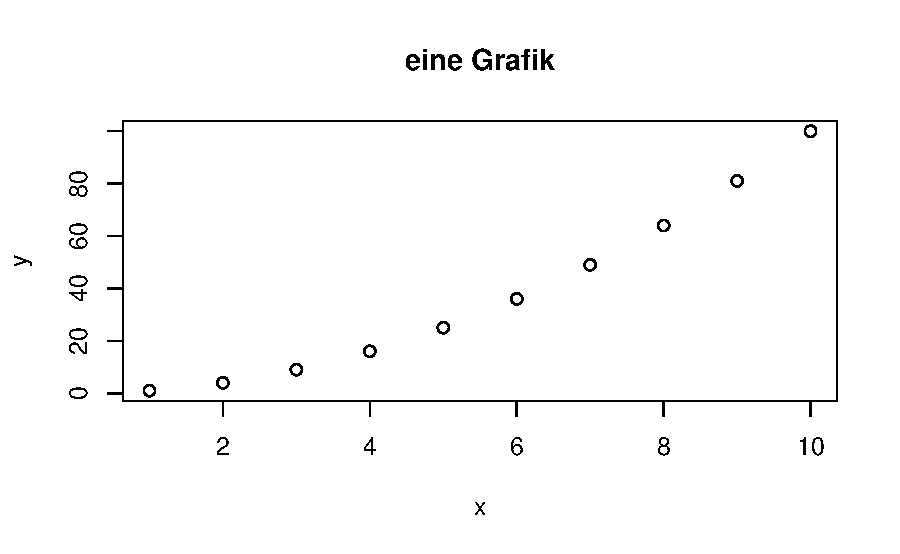
\includegraphics{bcd-styleguide_files/figure-pdf/unnamed-chunk-12-1.pdf}

\subsection{Nummerierte Beschriftungen und
Querverweise}\label{sec-Querverweise}

Um nummerierte Beschriftungen und Querverweise zu setzen, muss das
Zielelement mit einer ID versehen werden. Elementen (z. B. Code-Blöcke,
Grafiken, Überschriften) wird eine ID in geschweiften Klammern
übergeben, die ID muss innerhalb der geschweiften Klammer an erster
Stelle stehen und beginnt mit einer \texttt{\#}, gefolgt von einem
typabhängigen, reservierten Präfix. Anschließend folgt eine
beschreibende Zeichenkette, um das Zielelementen von anderen Elementen
des gleichen Typs zu unterscheiden. Auf diese Weise werden auch
Überschriften querverwiesen.

\begin{tcolorbox}[enhanced jigsaw, opacityback=0, rightrule=.15mm, leftrule=.75mm, left=2mm, colback=white, bottomrule=.15mm, colframe=quarto-callout-warning-color-frame, breakable, toprule=.15mm, arc=.35mm]
\begin{minipage}[t]{5.5mm}
\textcolor{quarto-callout-warning-color}{\faExclamationTriangle}
\end{minipage}%
\begin{minipage}[t]{\textwidth - 5.5mm}

\quartocalloutwrn{wrn-prefixlist} 

\vspace{-3mm}\textbf{Warning \ref*{wrn-prefixlist}: Hinweis reservierte Präfixe}\vspace{3mm}

In Quarto sind verschiedene Präfixe für die Erstellung von Querverweisen
reserviert: fig, tbl, lst, tip, nte, wrn, imp, cau, thm, lem, cor, prp,
cnj, def, exm, exr, sol, rem, eq, sec.

\end{minipage}%
\end{tcolorbox}

Der Callout Block vom Typ Hinweis im Abschnitt
Kapitel~\ref{sec-Verwendungsvorschlag} hat die ID
\texttt{\#nte-Beispiel}. Der Querverweis auf diesen Callout Block lautet
\texttt{@nte-Beispiel}: Beispiel~\ref{nte-Beispiel}.

(Siehe dazu:
\href{https://quarto.org/docs/authoring/cross-references.html}{Quarto
Cross References})

Grafiken erhalten das Präfix \texttt{fig}. In diesem Beispiel wird eine
ID vergeben sowie die Größe der Grafik mit der Option \texttt{width}
eingestellt:

\texttt{!{[}{]}(skript/00-bilder/working\_code\_CC0)\{\#fig-programmieren\ width="33\%"\}}

\begin{figure}

\centering{

\captionsetup{labelsep=none}
\includegraphics[width=0.33\textwidth,height=\textheight]{skript/00-bilder/working_code_CC0.pdf}

}

\caption{\label{fig-programmieren}}

\end{figure}%

Mit der ID kann ein Querverweis auf die Abbildung gesetzt werden:
\texttt{@fig-programmieren} erzeugt den Querverweis
Abbildung~\ref{fig-programmieren}.

\subsection{Grafiken}\label{grafiken}

Grafiken können lokal oder aus dem Internet eingebunden werden. Der
lokale Dateipfad wird ausgehend vom aktuellen Arbeitsverzeichnis
angegeben (siehe Kapitel~\ref{sec-Ordnerstruktur}).

\begin{description}
\tightlist
\item[Speicherort Grafiken]
\emph{Im Skript verwendete Grafiken werden im Unterordner
``skipt/00-bilder'' abgelegt.}

\emph{Für Aufgabenstellungen verwendete Grafiken werden im Unterordner
``aufgaben/00-bilder'' abgelegt.}
\end{description}

Die Syntax lautet:

\texttt{!{[}Grafiküberschrift{]}(skript/00-bilder/Dateiname\_Dateiname\ Dateiname.png)}\strut \\
\texttt{!{[}Grafiküberschrift{]}(https://beispiellink.de/einbild.png)}

\begin{tcolorbox}[enhanced jigsaw, opacityback=0, titlerule=0mm, bottomrule=.15mm, toptitle=1mm, toprule=.15mm, bottomtitle=1mm, rightrule=.15mm, leftrule=.75mm, left=2mm, colback=white, coltitle=black, colframe=quarto-callout-tip-color-frame, title=\textcolor{quarto-callout-tip-color}{\faLightbulb}\hspace{0.5em}{Tip \ref*{tip-arbeitsverzeichnis}: Arbeitsverzeichnis ermitteln}, arc=.35mm, breakable, opacitybacktitle=0.6, colbacktitle=quarto-callout-tip-color!10!white]

\quartocallouttip{tip-arbeitsverzeichnis} 

Das aktuelle Arbeitsverzeichnis kann mit einem Codeblock mit dem
entsprechenden Befehl angezeigt werden (hier ohne Ausgabe):

In R:

\begin{Shaded}
\begin{Highlighting}[]
\FunctionTok{print}\NormalTok{(}\FunctionTok{getwd}\NormalTok{())}
\end{Highlighting}
\end{Shaded}

In Python:

\begin{Shaded}
\begin{Highlighting}[]
\ImportTok{import}\NormalTok{ os}
\BuiltInTok{print}\NormalTok{(os.getcwd())}
\end{Highlighting}
\end{Shaded}

\end{tcolorbox}

\subsubsection{Grafikoptionen}\label{grafikoptionen}

Grafikoptionen können global im YAML-Header definiert werden.

\begin{verbatim}
---
cap-location: bottom
fig-align: center
---
\end{verbatim}

\begin{tcolorbox}[enhanced jigsaw, opacityback=0, rightrule=.15mm, leftrule=.75mm, left=2mm, colback=white, bottomrule=.15mm, colframe=quarto-callout-warning-color-frame, breakable, toprule=.15mm, arc=.35mm]
\begin{minipage}[t]{5.5mm}
\textcolor{quarto-callout-warning-color}{\faExclamationTriangle}
\end{minipage}%
\begin{minipage}[t]{\textwidth - 5.5mm}

\quartocalloutwrn{wrn-Beschriftung} 

\vspace{-3mm}\textbf{Warning \ref*{wrn-Beschriftung}: Grafiken ohne Beschriftung}\vspace{3mm}


\includegraphics[width=0.1\textwidth,height=\textheight]{skript/00-bilder/working_code_CC0.pdf}

Eine Grafik ohne Beschriftung oder \texttt{\#fig-ID} folgt der globalen
Einstellung nicht. Das obenstehende Bild steht in HTML linksbündig,
obwohl im YAML-Header \texttt{fig-align:\ center} konfiguriert ist.
Quarto unterscheidet intern zwischen unbeschrifteten Bildern (image) und
beschrifteten Grafiken (figure). Siehe
\url{https://github.com/quarto-dev/quarto-cli/issues/6509\#issuecomment-1677657369}.

\end{minipage}%
\end{tcolorbox}

Grafikoptionen können auch elementweise gesetzt werden. Optionen für
einzelne Grafiken werden in geschweiften Klammern übergeben und mehrere
Optionen durch Leerzeichen voneinander getrennt. Im folgenden Beispiel
wird eine \texttt{\#fig-ID} vergeben, ein Alternativtext mit
\texttt{fig-alt=""} angelegt, die Ausrichtung mit \texttt{fig-align=""}
linksbündig sowie die Größe der Grafik mit \texttt{width=""}
eingestellt. \texttt{width} stellt die Breite der Grafik ein, die Höhe
wird automatisch berechnet.

\texttt{!{[}Grafik\ mit\ elementweiser\ Option\ "left"{]}(skript/00-bilder/working\_code\_CC0.png)\{\#fig-Grafik-mit-Optionen\ fig-alt="Eine\ Person\ programmiert\ am\ Computer"\ fig-align="left"\ width="33\%"\}}

\begin{figure}


\includegraphics[width=0.33\textwidth,height=\textheight]{skript/00-bilder/working_code_CC0.png}

\caption{\label{fig-Grafik-mit-Optionen}Grafik mit elementweiser Option
``left''}

\end{figure}%

\begin{description}
\tightlist
\item[Grafiken]
\emph{Globale Einstellungen zentriert} \texttt{fig-align:\ center}

\emph{Beschriftung unterhalb} \texttt{cap-location:\ bottom}

\emph{Einbindung mit} \texttt{\#fig-ID} \emph{und Alternativtext}
\texttt{fig-alt="Alternativtext"} \emph{(ausgenommen dekorative
Grafiken)}
\end{description}

\emph{Dekorative Grafiken werden ohne \texttt{fig-ID} eingebunden und
erhalten ein Leerzeichen als Titel:
\texttt{{[}\&nbsp;{]}(skript/00-bilder/Dateipfad)}. Nicht gemeinfreie
Grafiken erhalten einen Lizenzhinweis nach der TULLU(BA)-Regel in einer
umrahmten Div \texttt{:::\ \{.border\}}.}

\begin{figure}[H]

{\centering 
\includegraphics[width=0.5\textwidth,height=\textheight]{bcd-styleguide_files/mediabag/skript/00-bilder/festmahl-PCL.pdf}

}

\caption{~}

\end{figure}%

Toast Dining Eating von OpenClipart-Vectors ist lizensiert unter
\href{https://pixabay.com/service/license-summary/}{Pixabay Content
License}. Das Werk ist abrufbar auf
\href{https://pixabay.com/vectors/toast-dining-eating-event-festive-153723/}{Pixabay}.
2013

\subsubsection{Nutzung von
Vektorgrafiken}\label{nutzung-von-vektorgrafiken}

Die Bausteine sind für den Export in HTML und PDF konzipiert. Der Export
von Grafiken nach PDF erfolgt über LaTeX und eine PDF-Renderengine.
Somit werden nur Formate unterstützt, die in LaTex und in PDF
unterstützt werden. Dies betrifft insbesondere

\begin{itemize}
\item
  Vektorgrafiken: Um Vektorgrafiken im Format SVG zu verarbeiten, wird
  die Bibliothek \texttt{Librsvg} benötigt. Siehe:
  \href{https://quarto.org/docs/prerelease/1.3/pdf.html}{Quarto: PDF
  Format Improvements}. Werden SVG-Grafiken mit Dateiendung (titel.svg)
  eingebunden, wandelt Quarto die Bilder automatisch in das PDF-Format
  um.
\item
  GIF: Das PDF-Format unterstützt animierte Bilddateien nicht bzw. nur
  in bestimmten Kombinationen aus Renderengine und PDF Reader. Quartos
  Standardengine TinyteX unterstützt animierte Bilddateien nicht.
\end{itemize}

Das für Grafiken verwendete Format kann global im YAML-Header definiert
werden.

\begin{verbatim}
format:
  html:
    default-image-extension: svg
  pdf:
    cite-method: biblatex
    default-image-extension: pdf
\end{verbatim}

Dann können Grafiken ohne Dateiendung eingebunden werden. Quarto lädt
dann automatisch das im YAML-Header definierte Dateiformat.
\texttt{!{[}Grafiküberschrift{]}(Unterordner/Dateiname\_ohne\ Dateiendung)}

\begin{tcolorbox}[enhanced jigsaw, opacityback=0, rightrule=.15mm, leftrule=.75mm, left=2mm, colback=white, bottomrule=.15mm, colframe=quarto-callout-warning-color-frame, breakable, toprule=.15mm, arc=.35mm]
\begin{minipage}[t]{5.5mm}
\textcolor{quarto-callout-warning-color}{\faExclamationTriangle}
\end{minipage}%
\begin{minipage}[t]{\textwidth - 5.5mm}

\vspace{-3mm}\textbf{Hinweis}\vspace{3mm}

Auf GitHub wandelt ein Skript alle SVG-Grafiken automatisch in PDF um.

\end{minipage}%
\end{tcolorbox}

\subsubsection{Flussdiagramme}\label{flussdiagramme}

Quarto unterstützt Graphviz und Mermaid zur Erzeugung von
\href{https://quarto.org/docs/authoring/markdown-basics.html\#diagrams}{Flussdiagrammen}.
Wird Mermaid verwendet, sollte im YAML-Header ein alternatives theme
konfiguriert werden, da das default theme sehr dunkle subgraphs erzeugt:

\begin{verbatim}
mermaid: 
  theme: neutral 
\end{verbatim}

\subsection{Videos und H5P-Elemente}\label{videos-und-h5p-elemente}

\begin{description}
\tightlist
\item[Speicherort von Videos]
\emph{Unterordner im Arbeitsverzeichnis ``videos''}
\end{description}

Die Syntax zur Einbindung von Videos lautet:

\begin{Shaded}
\begin{Highlighting}[]
\NormalTok{\# Allgemein}
\NormalTok{\{\{\textless{} video Dateipfad \textgreater{}\}\}}

\NormalTok{\# Beispiel}
\NormalTok{\{\{\textless{} video https://www.youtube.com/watch?v=EImihZVE0sA \textgreater{}\}\}}
\end{Highlighting}
\end{Shaded}

\url{https://www.youtube.com/watch?v=EImihZVE0sA}

Open Educational Resources concept: What is an OER? von UNESCO ist
lizensiert unter
\href{https://creativecommons.org/licenses/by/4.0/}{CC-BY}. Das Werk ist
abrufbar auf
\href{https://www.youtube.com/watch?v=EImihZVE0sA}{YouTube}.

~

\subsubsection*{H5P-Elemente}\label{h5p-elemente}
\addcontentsline{toc}{subsubsection}{H5P-Elemente}

H5P-Elemente können exportiert als all-in-one HTML file eingebunden
werden. Die Syntax lautet:

\begin{Shaded}
\begin{Highlighting}[]
\NormalTok{\{=html\}}
\NormalTok{\{\{\textless{} include Beispiel.html \textgreater{}\}\}}
\end{Highlighting}
\end{Shaded}

\subsection{Programmcode}\label{programmcode-1}

Code wird mit folgender Syntax eingebunden:

\begin{Shaded}
\begin{Highlighting}[]
\InformationTok{\textasciigrave{}\textasciigrave{}\textasciigrave{}\{python\}}
\InformationTok{print("Hallo Welt")}
\InformationTok{\textasciigrave{}\textasciigrave{}\textasciigrave{}}
\end{Highlighting}
\end{Shaded}

\begin{verbatim}
Hallo Welt
\end{verbatim}

Dabei können verschiedene \emph{Flags} gesetzt werden. Diese Flags
können entweder lokal in der Programmierumgebung oder aber global in der
yml-Datei gesetzt werden.

Mit \emph{\#\textbar{} echo: false} (standartmäßig \textbf{true}) kann
die Darstellung des Codes unterdrückt werden.

``` \{python\}\\
\#\textbar{} echo: false\\
print(``Hallo Welt'')\\
```

Im erzeugten Dokument wird dann nur die Ausgabe des Codes dargestellt
(die folgende Codezelle wird nicht dargestellt):

\begin{verbatim}
Hallo Welt
\end{verbatim}

Im Gegensatz dazu bestimmt \emph{\#\textbar{} output: false}
(standartmäßig \textbf{true}), dass der Code ohne Ausgabe dargestellt
werden soll.

\begin{Shaded}
\begin{Highlighting}[]
\InformationTok{\textasciigrave{}\textasciigrave{}\textasciigrave{}\{python\}}
\InformationTok{\#| output: false}
\InformationTok{print("Hallo Welt")}
\InformationTok{\textasciigrave{}\textasciigrave{}\textasciigrave{}}
\end{Highlighting}
\end{Shaded}

Mit \emph{\#\textbar{} output: asis} wird der Code ohne umschließende
Codezellen-Formatierung dargestellt:

\begin{Shaded}
\begin{Highlighting}[]
\BuiltInTok{print}\NormalTok{(}\StringTok{"Hallo Welt"}\NormalTok{)}
\end{Highlighting}
\end{Shaded}

Hallo Welt

Für die Code-Ausführung mit knitr (R-Code, Python-Code via reticulate)
bewirkt das Flag \emph{\#\textbar{} results: hold} eine zusammenhängende
Codeausführung.

\subsection{Python}

\begin{Shaded}
\begin{Highlighting}[]
\CommentTok{\# 2 Ausgaben mit Python}
\BuiltInTok{print}\NormalTok{(}\StringTok{"Ausgabe 1"}\NormalTok{)}
\end{Highlighting}
\end{Shaded}

\begin{verbatim}
Ausgabe 1
\end{verbatim}

\begin{Shaded}
\begin{Highlighting}[]
\BuiltInTok{print}\NormalTok{(}\StringTok{"Ausgabe 2"}\NormalTok{)}
\end{Highlighting}
\end{Shaded}

\begin{verbatim}
Ausgabe 2
\end{verbatim}

\subsection{Python results: hold}

\begin{Shaded}
\begin{Highlighting}[]
\CommentTok{\# 2 Ausgaben mit Python und gesetztem Flag results: hold}
\BuiltInTok{print}\NormalTok{(}\StringTok{"Ausgabe 1"}\NormalTok{)}
\BuiltInTok{print}\NormalTok{(}\StringTok{"Ausgabe 2"}\NormalTok{)}
\end{Highlighting}
\end{Shaded}

\begin{verbatim}
Ausgabe 1
Ausgabe 2
\end{verbatim}

\subsection{R}

\begin{Shaded}
\begin{Highlighting}[]
\CommentTok{\# 2 Ausgaben mit R}
\FunctionTok{print}\NormalTok{(}\StringTok{"Ausgabe 1"}\NormalTok{)}
\end{Highlighting}
\end{Shaded}

\begin{verbatim}
[1] "Ausgabe 1"
\end{verbatim}

\begin{Shaded}
\begin{Highlighting}[]
\FunctionTok{print}\NormalTok{(}\StringTok{"Ausgabe 2"}\NormalTok{)}
\end{Highlighting}
\end{Shaded}

\begin{verbatim}
[1] "Ausgabe 2"
\end{verbatim}

\subsection{R results: hold}

\begin{Shaded}
\begin{Highlighting}[]
\CommentTok{\# 2 Ausgaben mit R und gesetztem Flag results: hold}
\FunctionTok{print}\NormalTok{(}\StringTok{"Ausgabe 1"}\NormalTok{)}
\FunctionTok{print}\NormalTok{(}\StringTok{"Ausgabe 2"}\NormalTok{)}
\end{Highlighting}
\end{Shaded}

\begin{verbatim}
[1] "Ausgabe 1"
[1] "Ausgabe 2"
\end{verbatim}

Quarto bietet darüber hinaus weitere Konfigurationsmöglichkeiten für die
Präsentation von Programmcode
(\href{https://quarto.org/docs/output-formats/html-code.html\#overview}{siehe
Dokumentation}).

\subsubsection{Optionen für programmierte
Grafiken}\label{optionen-fuxfcr-programmierte-grafiken}

Die in den Bausteinen verwendeten Optionen zur Gestaltung programmierter
Grafiken sind im folgenden Block kurz erläutert.

\begin{verbatim}
#| fig-cap: "Beschriftung"
#| label: fig-ID "ID für Querverweise"
#| fig-alt: "Alternativtext"
#| fig-width: "Breite der Grafik als lokale Einstellung, in der Priorität über globaler Einstellung im YAML-Header"
#| fig-height: "Höhe der Grafik als lokale Einstellung, in der Priorität über globaler Einstellung im YAML-Header"
#| fig-asp: "Seitenverhältnis der Grafik als lokale Einstellung, in der Priorität über globaler Einstellung im YAML-Header"
\end{verbatim}

\section{Aufbau der Bausteine}\label{aufbau-der-bausteine}

Die Bausteine sind modular aufgebaut und bestehen aus drei Typen:
Werkzeugbausteinen, Methodenbausteinen und Anwendungsbausteinen.

\begin{itemize}
\item
  Werkzeugbausteine vermitteln den Umgang mit den Programmierumgebungen
  Python und R, die Entwicklung von Pseudocode und die rechtlichen
  Grundlagen des Datenmanagements.
\item
  Methodenbausteine vermitteln allgemeine methodische Grundlagen für die
  Datenanalyse wie die Analyse von Geodaten und Zeitreihen, Statistik,
  numerische Verfahren oder Datenfitting.
\item
  Anwendungsbausteine vermitteln fachspezifische Inhalte wie die
  Auswertung von Sensordaten, Stadt- und Verkehrsplanung,
  Branddatenanalyse.
\end{itemize}

Neben den fachlichen Inhalten umfassen Methoden- und Anwendungsbausteine
Codebeispiele für Python bzw. für R, die Studierenden die Bearbeitung
von Übungsaufgaben und Projekten in der jeweiligen Programmierumgebung
erlauben.

Die Bausteine folgen einem einheitlichen Aufbau:

\begin{itemize}
\item
  Voraussetzungen (eingebundene seperate Markdown-Datei)

  \begin{itemize}
  \item
    Inhaltliche Voraussetzungen
  \item
    vorher zu bearbeitende Bausteine
  \item
    verwendete Pakete und Datensätze / -quellen
  \item
    geschätzte Bearbeitungszeit
  \end{itemize}
\item
  Lernziele: Wissen, Kompetenzen, Leitfragen(eingebundene seperate
  Markdown-Datei.)
\item
  Inhalt (gerne abwechslungsreich gestalten)

  \begin{itemize}
  \item
    Theorie
  \item
    Beispiele
  \item
    Übungen
  \end{itemize}
\item
  Das Wichtigste (vielleicht als Video)
\item
  Lernzielkontrolle

  \begin{itemize}
  \item
    Kompetenzquiz (ggf. aufklappbarer Callout Block, Textverweis für
    PDF, polierte Lösungen evntl. via Lumi später entscheiden)
  \item
    Übungsaufgaben (kleine Projekte)
  \end{itemize}
\item
  Prüfungsaufgaben (ohne Lösungen)
\end{itemize}

\section{Ordnerstruktur}\label{sec-Ordnerstruktur}

\textbf{to do}

siehe Overleaf\ldots{} alles kleingeschrieben

\subsection{Sprache}\label{sprache}

Die Ansprache der Leser:innen erfolgt in der Höflichkeitsform ``Sie /
Ihr''. Gegendert wird mit dem Doppelpunkt: Er:Sie ist Busfahrer:in. Es
werden nur Personen gegendert. Nicht gegendert wird zum Beispiel: ``die
Anbieter von Plagiatserkennungssoftware''. Die Anbieter sind
Unternehmen.

Eine Alternative zum Gendern mit Doppelpunkt ist die Verlaufsform, z. B.
``Studierende''.

\subsection{Barrierefreiheit}\label{barrierefreiheit}

Siehe
\href{https://digitale-lehre.uni-siegen.de/wp-content/uploads/2023/09/Checkliste_Barrierefreiheit-in-der-digitalen-Lehre_Sept23.pdf}{Checklisten
Barrierefreiheit} Checklisten: Barrierefreiheit in der digitalen Lehre.
Hochschuldidaktik im digitalen Zeitalter.nrw; Kompetenzzentrum digitale
Barrierefreiheit.nrw. CC BY 4.0.

\section*{Quellenverzeichnis}\label{quellenverzeichnis}
\addcontentsline{toc}{section}{Quellenverzeichnis}

\printbibliography[heading=none]


\printbibliography[title=Quellen]


\end{document}
